 %美赛模板:正文部分

\documentclass[12pt]{article}  % 官方要求字号不小于 12 号,此处选择 12 号字体
% \linespread{1.1}
% \bibliographystyle{plain}
% 本模板不需要填写年份,以当前电脑时间自动生成
% 请在以下的方括号中填写队伍控制号
\usepackage[2102199]{easymcm}  % 载入 EasyMCM 模板文件
\problem{B}  % 请在此处填写题号
% \usepackage{mathptmx}  % 这是 Times 字体,中规中矩 
\usepackage{palatino}  % mathpazo 这palatino是 COMAP 官方杂志采用的更好看的 Palatino 字体,可替代以上的 mathptmx 宏包
\usepackage{pdfpages}
\usepackage{longtable}
\usepackage{tabu}
\usepackage{threeparttable}
\usepackage{listings}
\usepackage{paralist}
\graphicspath{{img/}}          % 此处{img/}为相对路径,注意加上“/”
 \let\itemize\compactitem
 \let\enditemize\endcompactitem

\newcommand{\upcite}[1]{\textsuperscript{\textsuperscript{\cite{#1}}}}
\title{Build an Army of Drones to Fight Wildfires}  % 标题

% 如需要修改题头(默认为 MCM/ICM),请使用以下命令(此处修改为 MCM)
%\renewcommand{\contest}{MCM}

 %文档开始
\begin{document}

% 此处填写摘要内容
\begin{abstract}
    
   Global warming, El Niño... With the emergence of various extreme climates,\textbf{Austral-ia's wildfires} occur more frequently. The greenhouse gases emitted after combustion have exacerbated global warming, which seems to have entered an endless loop. At the same time, hundreds of millions of lives have been killed in the fire, which makes us sad. In order to better control wildfires, we modeled the \textbf{distribution of drones} assisting in the observation to achieve the best balance between economy and efficiency.

Several models are established: Model I: Rasterized Multi-Objective Optimization Model; Model II: Model Verification Simulated by Poisson Process; Model III: Hovering Model Based on Tabu Search, etc.

For Model I: According to the \textbf{heat map} about distribution of fires in Victoria in recent years, we found that the main fire areas are the plains along the eastern coast. Inspired by weights and \textbf{Multi-Objective Optimization} algorithms, we built a brand-new model to find the best location for EOCs and draw up a suitable hover position and reconnaissance route for the drone. Based on the different positions of the fire site, calculate the maximum num-ber of two types of drones and their ratio. The results are shown in Figure 9.

For Model II: This model is actually a supplement to Model I. In the Model I, the fire only appeared in a small area, and there was a possibility of extreme fire events in the study area. Combining the data about nearly half a century and using the \textbf{Poisson Distribution }to obtain the probability and mathematical expectation, it can be concluded that 2.99431 ex-treme fire events may occur in the next ten years, which is approximately considered to be 3 times. After that, use the mobile EOC to deal with extreme fire events, and utilize the method of Model I to rebuild the drone network to find out what equipment costs need to be increased. Due to the diversity of the results, it will be shown in section 6.2.

For Model III: To tackle the problem of how to optimize the hover position of drones in different terrains, the \textbf{Tabu Search }algorithm (TS) is a good choice. Using the Tabu Search algorithm can make the hover position of the drones achieve the global optimal ef-fect under different terrain conditions. Since drone signals are severely interfered in urban areas, the reasonable distribution of EOCs enables it to quickly network to respond to sud-den urban fires. The obstruction of mountainous terrain restricts the drone's flying range. Therefore, dividing the area into blocks and managing them separately can effectively im-prove efficiency.

Finally, sensitivity analysis of the mathematical expectation of extreme fire events $\xi$ shows that our model is not sensitive to changes in $\xi$ , that is, it can be applied to areas with different extreme fire invents. Meanwhile, robustness of our model has also been tested. While adding 5\% random disturbance to $d_{k i}^{\alpha}$  and $d_{k i}^{\beta}$ , the maximum time error is 3.2657\%. The model can be considered stable. Afterwards, a Budget Request supported by our stable models has been written for CFA.


    % 美赛论文中无需注明关键字。若您一定要使用,
    % 请将以下两行的注释号 '%' 去除,以使其生效
    \vspace{5pt}  %mm	毫米	1 mm = 2.845 pt   pt 点	1 pt = 0.351 mm
    \textbf{Keywords}: Fighting Wildfires; Multi-Objective Optimization; Poisson Distribution; Tabu Search Algorithm; Sensitivity Analysis

\end{abstract}

\maketitle  % 生成 Summary Sheet

\tableofcontents  % 生成目录


% 正文开始
% Chapter 1: Introduction
\section{Introduction}

\subsection{Problem Background}
"Just like you, I was pain and fear when the fire destroyed the land and everything : life, houses, animals and trees. But for us aborigines, what the fire burns down is our memories, our holy land, and all the things that define our identity. " said by an aborigine. In recent years, the scale of fires in Australia has become larger and larger, causing huge economic and cultural losses. With the climate warming, the probability of fire is also greatly in-creased, so that it cannot be ignored anymore. We can see the fire situation in Australia from the figure below:

\begin{figure}[htbp]  %h此处,t页顶,b页底,p独立一页,浮动体出现的位置
\centering  %图表居中
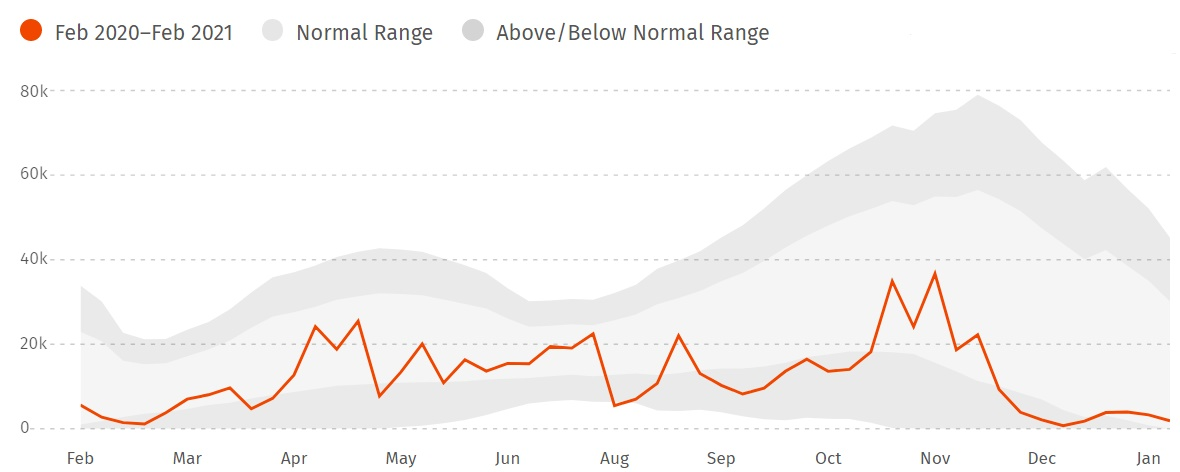
\includegraphics[width=.7\textwidth]{Fire_Situation.png} %图片的名称或者路径之中有空格会出问题 
\caption{Fire Situation in Australia (Feb 2020 - Feb 2021)} % 图片标题 
\label{fig:Fire Situation} % 图片标签,可以不写
\end{figure}

The data above comes from the website \textbf{GLOBAL FOREST WHATCH}\upcite{1}, The GFW Fires interactive map includes near real-time fire alerts from NASA and NOAA, real-time wind direction and air quality data, maps of concessions and forest cover, high-resolution satellite images, and geo-tagged social media conversations about where fires occur. 
As can be seen above: In Australia, the peak fire season typically begins in early January and lasts 45 weeks. There were 636,731 VIIRS fire alerts reported between February 2020 and February 2021. In response to the situation above, establishing a mathematical model driven by a swarm of drones to quickly deal with forest fires is very necessary and urgent.

\subsection{Restatement of the Problem}
Wildfire is a serious natural disaster with many complexities. Through in-depth analy-sis and research on the background of the problem, combined with the specific constraints given, the restate of the problem can be expressed as follows:

\begin{itemize}
\setlength{\parsep}{0ex} %段落间距
\setlength{\topsep}{2ex} %列表到上下文的垂直距离
\setlength{\itemsep}{1ex} %条目间距
\item Build a mathematical model to determine the optimal number and combination of SSA drones and Radio Repeater drones. The model should balance several factors.
\item Based on the model, explain how it adapts to the changing possibilities of extreme fire events in the next ten years.
\item Optimize the position of hovering VHF/UHF radio repeater drones based on an improved model for fires of different sizes on different terrains.
\item Considering the results obtained above, prepare one to two pages of annotated budget request and submit to the Victorian Government.
\end{itemize}

\subsection{Literature Review}
This question is mainly about mobilizing cluster drones to extinguish wildfires. In re-cent years, research on optimization algorithms for UAV(drone) cluster path planning is very hot, Generally, it can be divided into two parts, the \textbf{Swarms of UAVs' Path Planning Model} and the \textbf{Swarms of UAVs' Path Planning Optimization Algorithm}, this section mainly discusses the models that have been proposed.

\begin{itemize}
\setlength{\parsep}{0ex} %段落间距
\setlength{\topsep}{2ex} %列表到上下文的垂直距离
\setlength{\itemsep}{1ex} %条目间距  这三句如果删除就是各条贴在一起
\item First of all, in terms of the dimensionality of the space: In\upcite{2} HU et al. sets the plan-ning space to three dimensions. However, in order to simplify the model, more authors tend to consider the space as two dimensions\upcite{3}.
\item Secondly, in terms of the method of planning space: the commonly used methods in-clude Grid Method\upcite{4}, Road Sign Method, and Artificial Potential Fields Method.
\item Finally, the objective function of the UAV Cluster Path Planning Model generally uses flight distance, threat cost, etc. For example, Xu et al.\upcite{5} takes the weighted sum of threat cost and time cost as the optimization target. What's more, Constraints often in-clude self-constraints and environmental constraints, such as flight speed and geo-graphic altitude.
\item The strengths and weaknesses of the planning space can be visually presented and is shown below:
\end{itemize}

\begin{figure}[htbp]  %h此处,t页顶,b页底,p独立一页,浮动体出现的位置
\centering  %图表居中
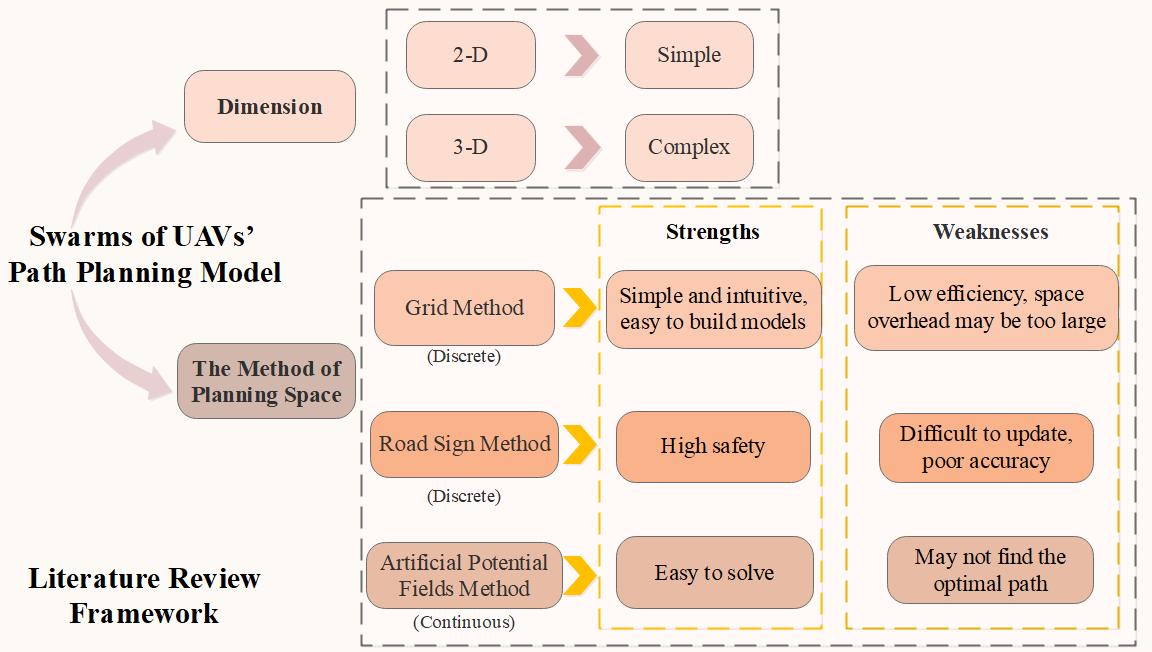
\includegraphics[width=.85\textwidth]{Literature_Review.png} %图片的名称或者路径之中有空格会出问题 
\caption{Literature Review Framework} % 图片标题 
\end{figure}

\subsection{Our Work}
The problem requires us to fight fires by optimizing the locations of two type of drones. Our work mainly includes the following:
\begin{enumerate}[\bfseries 1.]
    \setlength{\parsep}{0ex} %段落间距
    \setlength{\topsep}{0.5pt} %列表到上下文的垂直距离
    \setlength{\itemsep}{0.5pt} %条目间距
    \item Based on the data of wildfires, a rasterized Multi-Objective Optimization Model is established;
    \item The mixture of the two drones is given and the extreme fire events is considered;
    \item Based on the verification model simulated by Poisson process and the hovering model based on Tabu Search, this article effectively demonstrates the validity and applicability.
\end{enumerate}
In order to avoid complicated description, intuitively reflect our work process, the flow chart is shown in Figure 3:

\begin{figure}[htbp]  %h此处,t页顶,b页底,p独立一页,浮动体出现的位置
\centering  %图表居中
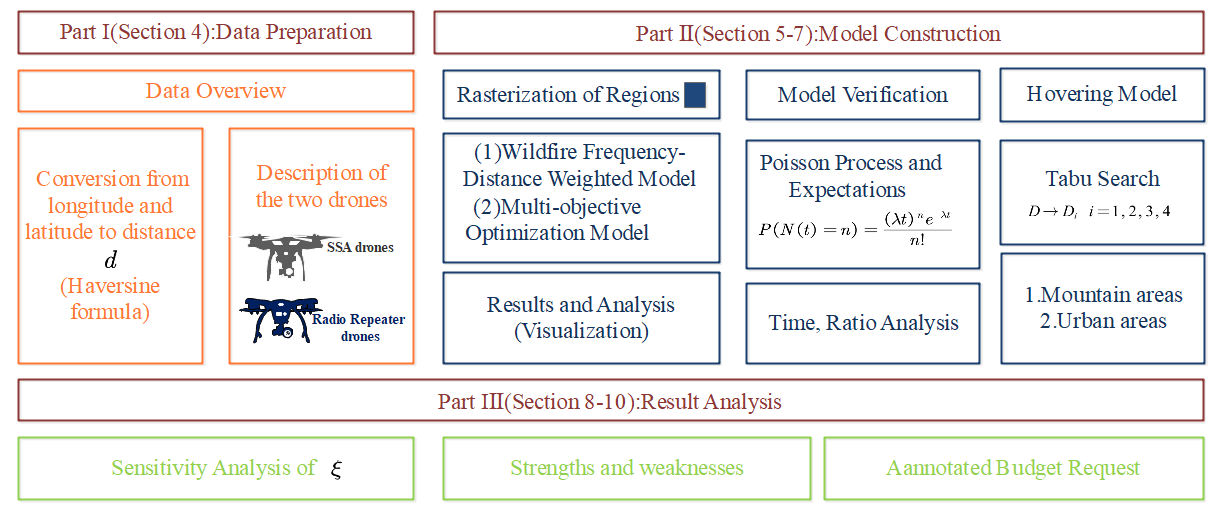
\includegraphics[width=.9\textwidth]{Flow_Chart.png} %图片的名称或者路径之中有空格会出问题 
\caption{Flow Chart of Our Work} % 图片标题 
\end{figure}
\vspace{-0.8cm}

\section{Assumptions and Explanations}
Considering that practical problems always contain many complex factors, first of all, we need to make reasonable assumptions to simplify the model, and each hypothesis is closely followed by its corresponding explanation:

\begin{enumerate}[\bfseries \textit{Assumption} 1:]
	\item \textbf{Only the influence of terrain on the drone is considered, and other factors such as temperature, humidity, and atmosphere are ignored.}\\
	\textbf{\textit{Explanation:}}The UAV's radiation communication range is only affected by terrain factors, and other factors are minimal. In fact, these factors affect each other, but in order to simplify the model ,we ignore the interactions between these factors.
	\item \textbf{The location of the EOC can be deployed around the fire due to an emergency.}\\
	\textbf{\textit{Explanation:}}The position of the EOC is not clearly given in the question. So, we assume that EOC can be set in a fire-free area around the wildfire site, since the glossary of the problem said that mobile EOC can be deployed near the site of an emergency.
	\item \textbf{The "boots-on-the-ground" forward teams can be approximated as near the fire site.}\\
	\textbf{\textit{Explanation:}}The actual movement of the team is very complicated, and it is difficult to accurately calculate its position. Therefore, it is assumed that the squad is near the fire field and the drone arrives at the fire field to establish a connection with the squad.
	\item \textbf{The collected data can be considered reliable and can reflect the changing laws of the Victorian wildfire.}\\
	\textbf{\textit{Explanation:}}The historical Victorian wildfire data, latitude, longitude and other data come from authoritative websites, such as the official website of FEC in Australia and NASA, with high accuracy.
\end{enumerate}
Additional assumptions are made to simplify analysis for individual sections. These assumptions will be discussed at the appropriate locations.

\section{Notations}
Some important mathematical notations used in this paper are listed in Table 1. 
\begin{table}[htbp]
\begin{center}
\caption{Notations used in this paper}
\begin{tabular}{c l}
\toprule[2pt]
\multicolumn{1}{m{3cm}}{\centering Symbol}
&\multicolumn{1}{m{8cm}}{\centering Description }\\
\midrule
$x_i$& Longitude within the i-th Wildfire Grid \\
$y_i$& Latitude within the i-th Wildfire Grid \\
$\varOmega _i$& The area of the i-th grid\\
$d_{ki}$& the distance $d_{ki}$ between the k-th roaming grid and the i-th grid \\
$SC_k$ & Score for evaluating the k-th wildfire grid \\
\vspace{5pt}%公式间有点挤,空一些
$x^{( \alpha )}_{ki}$ & the $SSA_\alpha$ drone sent by the k-th EOC to the i-th wild-fire grid\\
\vspace{3pt}
$x^{( \beta )}_{ki}$ & the $RR_\beta$ drone sent by the k-th EOC to the i-th wildfire grid\\
$t_{fly}^{\delta}$ & The flight time of drones\\
\bottomrule[2pt]
\end{tabular}\label{tb:notation}
 \begin{tablenotes}
        \footnotesize
        \item[*] *There are some variables that are not listed here and will be discussed in detail in each section. %此处加入注释*信息
      \end{tablenotes}
\end{center}
\end{table}
\vspace{-1cm}%在\end{table}下加一行\vspace{-1cm} 其中-1的作用是缩短与下方文字距离的 切记!必须是负数

\section{Model Preparation}
\subsection{Data Overview}
The question did not provide us with data directly, so we need to consider which data to collect in the model building. Through the analysis of the problem, we need to collect the relevant information of Victoria, Australia, such as \textbf{latitude and longitude, altitude, number of wildfires} and so on. Due to the large amount of data, it is not convenient to list them all, so visualizing the data for display is a good method.

\subsubsection{Data Collection}
The official website of FEC in Victoria, Australia was queried and lots of data about wildfires were obtained. And other data sources are shown in Table 2.

\begin{table}[htbp]
\begin{center}
\caption{Data and Database Websites}
\resizebox{\textwidth}{!}
{\begin{tabular}{c c}
\toprule[2pt]
\multicolumn{1}{m{5cm}}{\centering \textbf{Database Names}}
&\multicolumn{1}{m{10cm}}{\centering \textbf{Database Websites} }\\ %m后面是列宽
\midrule
Fire Alerts& https://www.globalforestwatch.org/map/ \\
Altitude & https://search.earthdata.nasa.gov/search \\
Latitude and Longitude & https://www.kaggle.com/carlosparadis/\\ 
Google Scholar & https://scholar.google.com/ \\
Maps& \copyright{} 2021 Mapbox \copyright{} OpenStreetMap\\
\bottomrule[2pt]
\end{tabular}}
\end{center}
\end{table}

\subsubsection{Data Screening}
Judging from the map of Victoria in Figure 4 (right), the eastern region is mainly forest, while the western region is almost no forest. Furthermore, to demonstrate better the situa-tion of wildfires, we plot over a heat map in Figure 4 (left).
Considering the heat map we made, it shows the number of wildfires in various states of Victoria from 2012 to 2021, the darker the color, the greater number of fires. Although fires have also occurred in the western region, the number of eastern regions is much higher than that in the western region. 

\begin{figure}[htbp]
    \centering    
    \subfigure[Data Screening(left)]{				% 图片1([]内为子图标题)						
    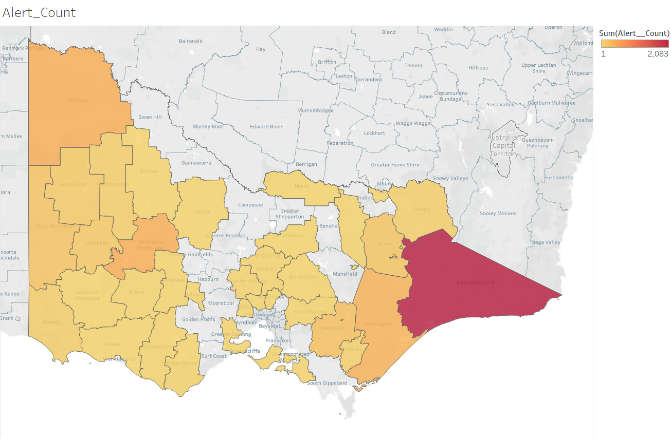
\includegraphics[width=0.45\textwidth]{Data_Screening(1).png}}			  % 子图1的图片宽度 不能空行
    \subfigure[Data Screening(right)]{				% 图片2
    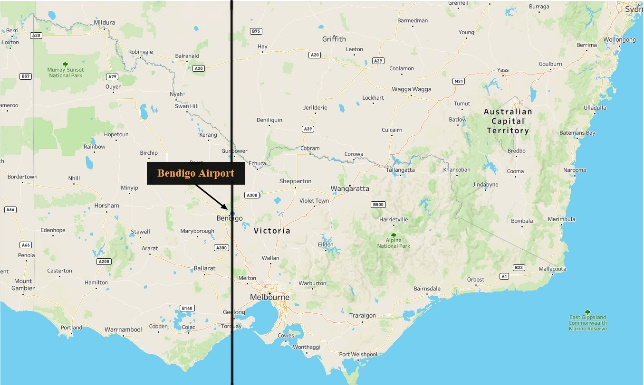
\includegraphics[width=0.45\textwidth]{Data_Screening(2).png}}
	\caption{Data Screening} % 图片标题 
\end{figure}

\begin{enumerate}[\bfseries 1.]
    \setlength{\parsep}{0ex} %段落间距
    \setlength{\topsep}{0ex} %列表到上下文的垂直距离
    \setlength{\itemsep}{0ex} %条目间距
    \item The analysis of locations of hovering VHF/UHF radio-repeater drones for fires can be more accurate if we have more complete data;
    \item The assumption that the "boots-on-the-ground" forward teams can be approximated as near the fire site is a bit idealized. If the trajectory of the team is taken into account, a more practical model and results can be obtained.
    \item Some approximate analysis methods are applied to model other places, which may lead to the situation that not to be the most optimal.
\end{enumerate}

% 参考文献,此处以 MLA 引用格式为例
\clearpage   %另起一页继续写。这时,你最好使用“\clearpage” 
\begin{thebibliography}{99}
    \bibitem{1} GLOBAL FOREST WHATCH OF AUSTRALIA https://www.globalforestwatch.org/topics/fires/?topic=fires\#footer
	\bibitem{2} HU Teng, LIU Zhanjun, LIU Yang, et al. 3D reconnaissance path planning of multiple UAVs. Journal of Systems Engineering and Electronics, 2019, 41(7): 1551-1559.
	\bibitem{3} BASBOUS B. 2D UAV path planning with radar threatening areas using simulated an-nealing algorithm for event detection. The 2018 International Conference on Artificial Intelligence and Data Processing. Malatya, Turkey: IEEE,2018: 1-7.
	\bibitem{4} WANG W F, WU Y C, ZHANG X. Research of the unit decomposing traversal method based on grid method of the mobile robot. Techniques of Automation and Applications, 2013, 32(11): 34-38.
	\bibitem{5} XU Jian, ZHOU Deyun, HUANG He. Multi UAV path planning based on improved ge-netic algorithm. Aeronautical Computing Technique, 2009, 39(4): 43-46.

\end{thebibliography}
% \includepdf[pages={1,2}]{Memo.pdf} 

\end{document}  % 结束